
%\documentclass{article}
\documentclass[tikz]{standalone}

\usepackage{pgf}
\usepackage{tikz}
\usetikzlibrary{arrows,automata,positioning}
%\usepackage[latin1]{inputenc}
\usepackage{verbatim}
\usepackage{graphicx}

\begin{document}

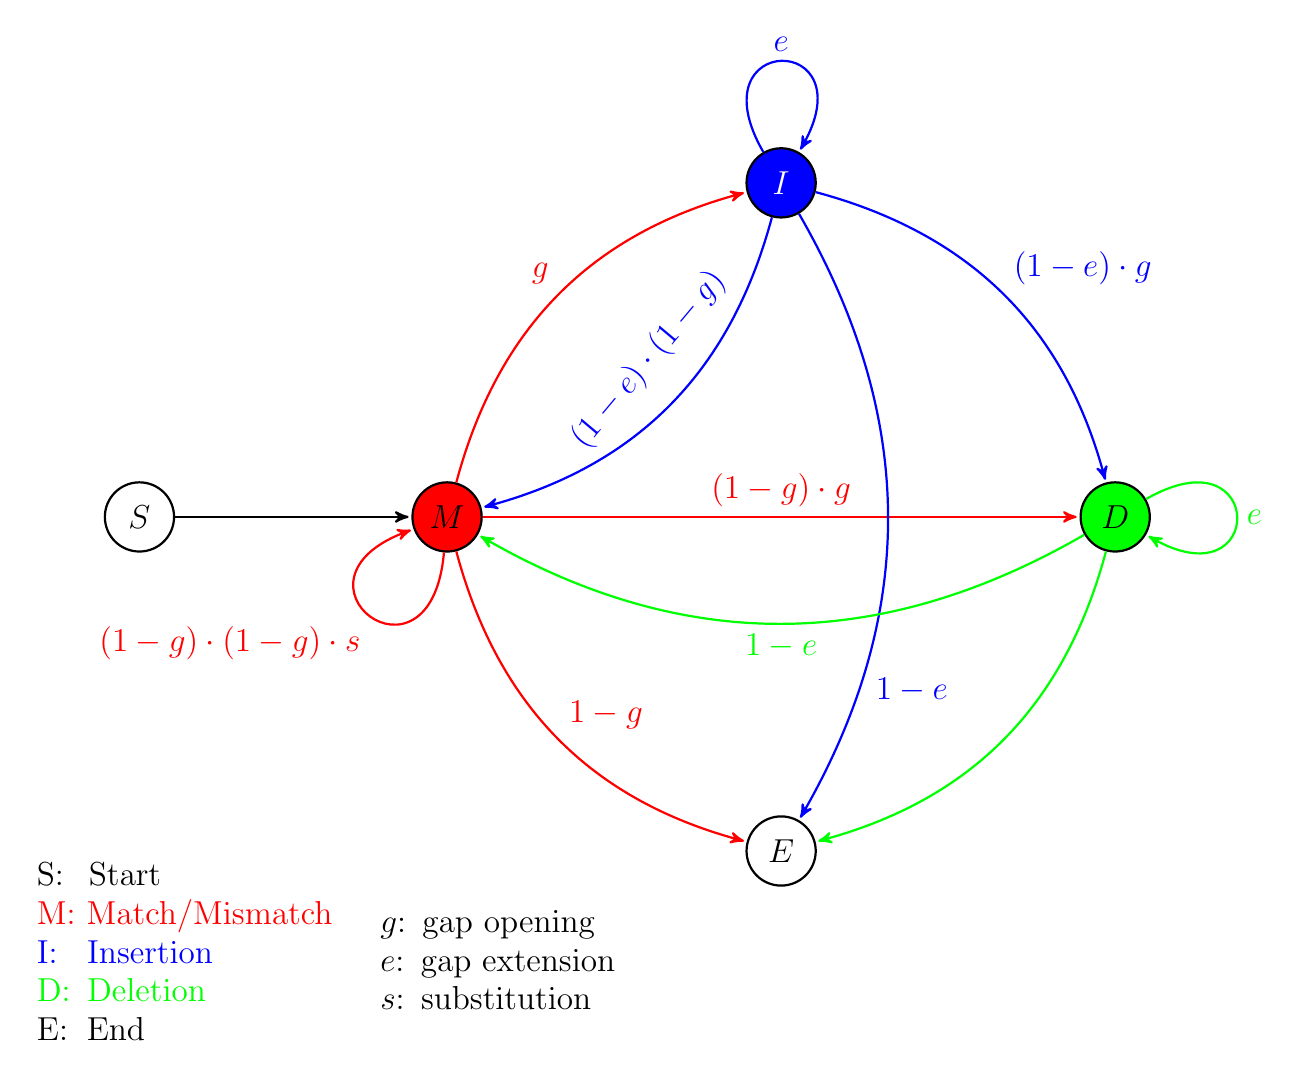
\begin{tikzpicture}[->,>=stealth',shorten >=1pt,auto,node distance=6cm,thick]
  \tikzstyle{every node}=[font=\large]

  \node[state]         (S)					  {$S$};
  \node[state,fill=red]		   (M) [right=30mm of S]       {$M$};
  \node[state,fill=blue,text=white]         (I) [above right of=M] {$I$};
  \node[state]         (E) [below right of=M] {$E$};
  \node[state,fill=green]         (D) [below right of=I] {$D$};

  \path (S) edge 			  node {}	(M)
  		(M) edge [red,out=265,in=200,looseness=10]  node [midway] {$(1-g)\cdot(1-g)\cdot s$} (M)
  			edge [red,bend left]  node {$g$} (I)
            edge [red]        node {$(1-g)\cdot g$} (D)
            edge [red,bend right] node {$1-g$}	(E)
        (I) edge [blue,out=120,in=60,looseness=10] node {$e$} (I)
            edge [blue,bend left]  node [rotate=50, above=1em] {$(1-e)\cdot (1-g)$} (M)
            edge [blue,bend left]  node {$(1-e) \cdot g $} (D)
            edge [blue,bend left] node [near end] {$1-e$} (E)
        (D) edge [green,out=30,in=330,looseness=10] node {$e$} (D)
        	edge [green,bend left]  node {$1-e$} (M)
        	edge [green,bend left]  node {}	(E);

  \node[text width=4cm, below left=-3mm and 50mm of E] (T1) {S: \hspace{0.4mm} Start\\
  \textcolor{red}{M: Match/Mismatch}\\ \textcolor{blue}{I: \hspace{1mm} Insertion}\\
  \textcolor{green}{D: \hspace{0.7mm}Deletion}\\ E: \hspace{1mm}End};
  \node[text width=5cm, right=1mm of T1] (T2) {\\ $g$: gap opening\\ $e$: gap extension\\ $s$: substitution};

\end{tikzpicture}


\end{document}
